\documentclass[tikz,border=2pt]{standalone}
\usepackage{amsmath,amssymb}
\usepackage{tikz}
\usetikzlibrary{arrows.meta,positioning}

\begin{document}
% Task quotas: agent 1 must take exactly 2 tasks and agent 2 exactly 1 of the three tasks;
% equivalently split agent 1 into two copies and solve a square assignment problem.
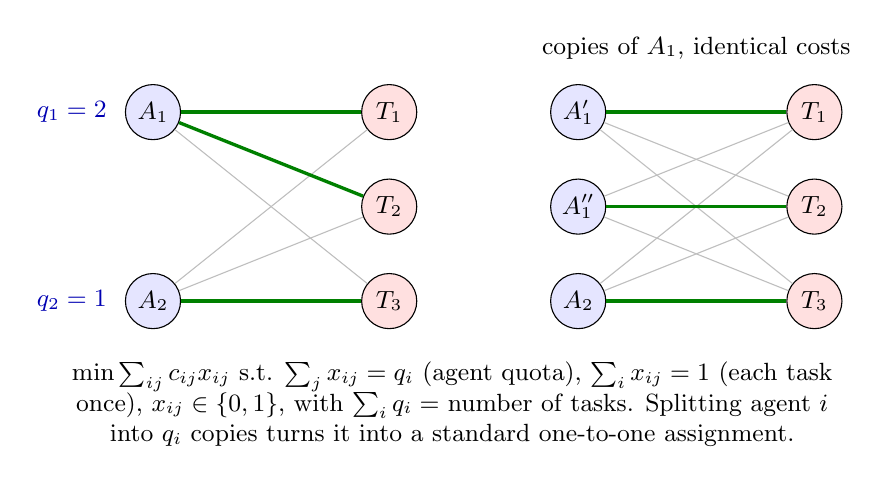
\begin{tikzpicture}[every node/.style={font=\small}, v/.style={draw, circle, fill=blue!10, minimum size=7mm, inner sep=0pt}, w/.style={draw, circle, fill=red!12, minimum size=7mm, inner sep=0pt}]
	\node[v] (a1) at (0,1.2) {$A_1$}; \node[v] (a2) at (0,-1.2) {$A_2$};
	\foreach \j in {1,2,3} {\node[w] (t\j) at (3.0,{2.4-1.2*\j}) {$T_\j$};}
	\foreach \i/\j in {1/1, 1/2, 1/3, 2/1, 2/2, 2/3} {\draw[gray!50] (a\i) -- (t\j);}
	\draw[green!50!black, very thick] (a1) -- (t1); \draw[green!50!black, very thick] (a1) -- (t2); \draw[green!50!black, very thick] (a2) -- (t3);
	\node[blue!70!black, left=3pt of a1] {$q_1=2$};
	\node[blue!70!black, left=3pt of a2] {$q_2=1$};
	\begin{scope}[xshift=5.4cm]
		\node[v] (b1) at (0,1.2) {$A_1'$}; \node[v] (b2) at (0,0) {$A_1''$}; \node[v] (b3) at (0,-1.2) {$A_2$};
		\foreach \j in {1,2,3} {\node[w] (u\j) at (3.0,{2.4-1.2*\j}) {$T_\j$};}
		\foreach \i/\j in {1/2, 1/3, 2/1, 2/3, 3/1, 3/2} {\draw[gray!50] (b\i) -- (u\j);}
		\draw[green!50!black, very thick] (b1) -- (u1); \draw[green!50!black, very thick] (b2) -- (u2); \draw[green!50!black, very thick] (b3) -- (u3);
		\node[anchor=south] at (1.5,1.75) {copies of $A_1$, identical costs};
	\end{scope}
	\node[anchor=north, align=flush center, text width=10cm] at (3.8,-1.85) {$\min\sum_{ij}c_{ij}x_{ij}$ s.t. $\sum_jx_{ij}=q_i$ (agent quota), $\sum_ix_{ij}=1$ (each task once), $x_{ij}\in\{0,1\}$, with $\sum_iq_i=$ number of tasks. Splitting agent $i$ into $q_i$ copies turns it into a standard one-to-one assignment.};
\end{tikzpicture}
\end{document}
